\documentclass[]{article}
\usepackage{lmodern}
\usepackage{amssymb,amsmath}
\usepackage{ifxetex,ifluatex}
\usepackage{fixltx2e} % provides \textsubscript
\ifnum 0\ifxetex 1\fi\ifluatex 1\fi=0 % if pdftex
  \usepackage[T1]{fontenc}
  \usepackage[utf8]{inputenc}
\else % if luatex or xelatex
  \ifxetex
    \usepackage{mathspec}
  \else
    \usepackage{fontspec}
  \fi
  \defaultfontfeatures{Ligatures=TeX,Scale=MatchLowercase}
\fi
% use upquote if available, for straight quotes in verbatim environments
\IfFileExists{upquote.sty}{\usepackage{upquote}}{}
% use microtype if available
\IfFileExists{microtype.sty}{%
\usepackage{microtype}
\UseMicrotypeSet[protrusion]{basicmath} % disable protrusion for tt fonts
}{}
\usepackage[margin=1in]{geometry}
\usepackage{hyperref}
\hypersetup{unicode=true,
            pdftitle={Curs Biostatistica 2017 - Laborator 9 \& 10},
            pdfborder={0 0 0},
            breaklinks=true}
\urlstyle{same}  % don't use monospace font for urls
\usepackage{graphicx,grffile}
\makeatletter
\def\maxwidth{\ifdim\Gin@nat@width>\linewidth\linewidth\else\Gin@nat@width\fi}
\def\maxheight{\ifdim\Gin@nat@height>\textheight\textheight\else\Gin@nat@height\fi}
\makeatother
% Scale images if necessary, so that they will not overflow the page
% margins by default, and it is still possible to overwrite the defaults
% using explicit options in \includegraphics[width, height, ...]{}
\setkeys{Gin}{width=\maxwidth,height=\maxheight,keepaspectratio}
\IfFileExists{parskip.sty}{%
\usepackage{parskip}
}{% else
\setlength{\parindent}{0pt}
\setlength{\parskip}{6pt plus 2pt minus 1pt}
}
\setlength{\emergencystretch}{3em}  % prevent overfull lines
\providecommand{\tightlist}{%
  \setlength{\itemsep}{0pt}\setlength{\parskip}{0pt}}
\setcounter{secnumdepth}{5}
% Redefines (sub)paragraphs to behave more like sections
\ifx\paragraph\undefined\else
\let\oldparagraph\paragraph
\renewcommand{\paragraph}[1]{\oldparagraph{#1}\mbox{}}
\fi
\ifx\subparagraph\undefined\else
\let\oldsubparagraph\subparagraph
\renewcommand{\subparagraph}[1]{\oldsubparagraph{#1}\mbox{}}
\fi

%%% Use protect on footnotes to avoid problems with footnotes in titles
\let\rmarkdownfootnote\footnote%
\def\footnote{\protect\rmarkdownfootnote}

%%% Change title format to be more compact
\usepackage{titling}

% Create subtitle command for use in maketitle
\newcommand{\subtitle}[1]{
  \posttitle{
    \begin{center}\large#1\end{center}
    }
}

\setlength{\droptitle}{-2em}
  \title{Curs Biostatistica 2017 - Laborator 9 \& 10}
  \pretitle{\vspace{\droptitle}\centering\huge}
  \posttitle{\par}
\subtitle{Regresie}
  \author{}
  \preauthor{}\postauthor{}
  \date{}
  \predate{}\postdate{}

\usepackage{booktabs}
\usepackage{longtable}
\usepackage{framed,color}
\definecolor{shadecolor}{RGB}{248,248,248}

\ifxetex
  \usepackage{letltxmacro}
  \setlength{\XeTeXLinkMargin}{1pt}
  \LetLtxMacro\SavedIncludeGraphics\includegraphics
  \def\includegraphics#1#{% #1 catches optional stuff (star/opt. arg.)
    \IncludeGraphicsAux{#1}%
  }%
  \newcommand*{\IncludeGraphicsAux}[2]{%
    \XeTeXLinkBox{%
      \SavedIncludeGraphics#1{#2}%
    }%
  }%
\fi

\newenvironment{rmdblock}[1]
  {\begin{shaded*}
  \begin{itemize}
  \renewcommand{\labelitemi}{
    \raisebox{-.7\height}[0pt][0pt]{
      {\setkeys{Gin}{width=2em,keepaspectratio}\includegraphics{images/icons/#1}}
    }
  }
  \item
  }
  {
  \end{itemize}
  \end{shaded*}
  }
\newenvironment{rmdcaution}
  {\begin{rmdblock}{caution}}
  {\end{rmdblock}}
\newenvironment{rmdinsight}
  {\begin{rmdblock}{insight}}
  {\end{rmdblock}}
\newenvironment{rmdexercise}
  {\begin{rmdblock}{exercise}}
  {\end{rmdblock}}
\newenvironment{rmdtip}
  {\begin{rmdblock}{tip}}
  {\end{rmdblock}}

\begin{document}
\maketitle

{
\setcounter{tocdepth}{2}
\tableofcontents
}
\section{Regresie liniară multiplă}\label{regresie-liniara-multipla}

\begin{center}\rule{0.5\linewidth}{\linethickness}\end{center}

\begin{center}\rule{0.5\linewidth}{\linethickness}\end{center}

\subsection{Introducere}\label{introducere}

Modelul de regresie liniară multiplă reprezintă o generalizare a
modelului de regresie simplă. Dacă în regresia liniară simplă se folosea
o singură variabilă predictor \(X\) ca să explice variabila răspuns
\(Y\), în modelul de regresie liniară multiplă se folosesc mai multe
variabile predictor \(X_1,\ldots,X_k\) pentru a explica răspunsul \(Y\):

\[
\mathbb{E}[Y|X_1 = x_1, \ldots, X_k=x_x]=\beta_0+\beta_1x_1+\beta_2x_2+\ldots+\beta_kx_k
\] sau altfel scris

\[
Y = \beta_0 + \beta_1 X_1 + \ldots + \beta_k X_k + \varepsilon.
\]

Date fiind observațiile actuale, cu alte cuvinte dat fiind un eșantion
\((X_{11},\ldots,X_{1k},Y_1),\ldots,(X_{n1},\ldots,X_{nk},Y_n)\) al lui
\((X_1,\ldots,X_k,Y)\), unde \(X_{ij}\) reprezintă a \(i\)-a observație
a predictorului \(X_j\), modelul se poate scrie

\[
y_i = \beta_0+\beta_1x_{i1}+\beta_2x_{i2}+\ldots+\beta_kx_{ik}+\varepsilon_i, \quad i = 1,\ldots,n
\]

a cărui formă compactă (matriceală) este

\[
\mathbf{Y}=\mathbf{X}\boldsymbol\beta+\boldsymbol\varepsilon
\]

\begin{itemize}
\tightlist
\item
  \(\mathbf{X}\) este \emph{matricea de design}
\end{itemize}

\[
\mathbf{X}=\begin{pmatrix}
1 & X_{11} & \cdots & X_{1k}\\
\vdots & \vdots & \ddots & \vdots\\
1 & X_{n1} & \cdots & X_{nk}
\end{pmatrix}_{n\times(k+1)}
\]

\begin{itemize}
\tightlist
\item
  \(\mathbf{Y}\) este \emph{vectorul răspuns}, \(\boldsymbol\beta\) este
  \emph{vectorul coeficienților} iar \(\boldsymbol\varepsilon\) este
  \emph{vectorul eroare}
\end{itemize}

\[
\mathbf{Y}=\begin{pmatrix}
Y_1 \\
\vdots \\
Y_n
\end{pmatrix}_{n\times 1},\quad\boldsymbol\beta=\begin{pmatrix}
\beta_0 \\
\beta_1 \\
\vdots \\
\beta_k
\end{pmatrix}_{(k+1)\times 1}\text{ și }\quad
\boldsymbol\varepsilon=\begin{pmatrix}
\varepsilon_1 \\
\vdots \\
\varepsilon_n
\end{pmatrix}_{n\times 1}.
\]

\BeginKnitrBlock{rmdinsight}

Să observăm că pentru \(k=1\) modelul se reduce la regresia liniară
simplă. În acest caz:

\[
\mathbf{X}=\begin{pmatrix}
1 & X_{11}\\
\vdots & \vdots\\
1 & X_{n1}
\end{pmatrix}_{n\times2}\text{ și }\quad \beta=\begin{pmatrix}
\beta_0 \\
\beta_1 
\end{pmatrix}_{2\times 1}
\]

\EndKnitrBlock{rmdinsight}

\emph{Suma abaterilor pătratice reziduale} pentru modelul de regresie
liniară multiplă este

\[
RSS(\boldsymbol\beta)=\sum_{i=1}^n(Y_i-\beta_0-\beta_1X_{i1}-\ldots-\beta_kX_{ik})^2=(\mathbf{Y}-\mathbf{X}\boldsymbol{\beta})^T(\mathbf{Y}-\mathbf{X}\boldsymbol{\beta})
\]

ceea ce conduce la \emph{sistemul de ecuații normale}

\[
\mathbf{X}^\intercal\mathbf{X}\hat{\boldsymbol{\beta}}=\mathbf{X}^\intercal\mathbf{Y}
\]

a cărui soluție, dat fiind că \(\mathbf{X}^\intercal\mathbf{X}\) este
inversabilă, este

\[
\hat{\boldsymbol{\beta}}=(\mathbf{X}^\intercal\mathbf{X})^{-1}\mathbf{X}^\intercal\mathbf{Y}
\]

Odată ce avem estimatorul \(\hat{\boldsymbol{\beta}}\) , putem defini:

\begin{itemize}
\tightlist
\item
  \emph{valorile prognozate} (\emph{fitted values})
  \(\hat Y_1,\ldots,\hat Y_n\) (valorile verticale pe hiperplanul de
  regresie), unde
\end{itemize}

\[
\hat Y_i=\hat\beta_0+\hat\beta_1X_{i1}+\cdots+\hat\beta_kX_{ik},\quad i=1,\ldots,n
\]

și sub formă matriceală

\[
\hat{\mathbf{Y}}=\mathbf{X}\hat{\boldsymbol{\beta}}=\mathbf{X}(\mathbf{X}^\intercal\mathbf{X})^{-1}\mathbf{X}^\intercal\mathbf{Y}=\mathbf{H}\mathbf{Y}
\]

unde
\(\mathbf{H}=\mathbf{X}(\mathbf{X}^\intercal\mathbf{X})^{-1}\mathbf{X}^\intercal\)
se numește \emph{matricea căciulă} (\emph{hat matrix}) și reprezintă
proiecția ortogonală a lui \(\mathbf{Y}\) în spațiul generat de
\(\mathbf{X}\).

\begin{itemize}
\tightlist
\item
  \emph{reziduurile estimate} (\emph{estimated residuals})
  \(\hat \varepsilon_1,\ldots,\hat \varepsilon_n\), unde
\end{itemize}

\[
\hat\varepsilon_i=Y_i-\hat Y_i,\quad i=1,\ldots,n
\]

și sub formă matriceală

\[
\hat{\boldsymbol\varepsilon} = \boldsymbol Y - \hat{\boldsymbol Y} = (\boldsymbol I-\boldsymbol H)\boldsymbol Y
\]

\begin{figure}

{\centering 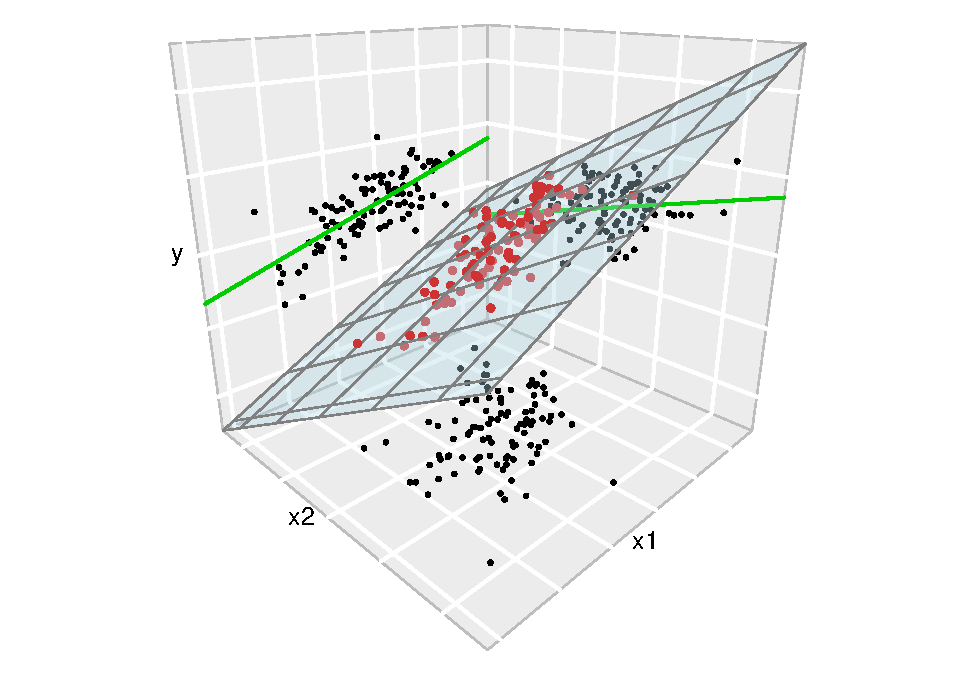
\includegraphics[width=0.9\linewidth]{Lab_9_10_files/figure-latex/unnamed-chunk-3-1} 

}

\caption{Planul de regresie (albastru) si relatia cu regresiile liniare simple (liniile verzi). Punctele rosii reprezinta un esantion pentru $(X_1,X_2,Y)$ iar punctele negre sunt subesantioane pentru $(X_1,X_2)$ (la baza), $(X_1,Y)$ (stanga) si $(X_2,Y)$ (dreapta).}\label{fig:unnamed-chunk-3}
\end{figure}

\subsection{Exemplul 1}\label{exemplul-1}


\end{document}
